% vim: spelllang=fr

\documentclass[../main.tex]{subfiles}
\graphicspath{{\subfix{../Figures/Chap2/}}}
\begin{document}

\begin{itshape}
Ce deuxième chapitre porte de l'approche directe consistant en l'application d'un algorithme de détection et de suivi des cyclones tropicaux dans les modèles
comme façon de caractériser l'activité cyclonique simulée, ainsi que la façon dont les modèles représentent ces phénomènes. Un cas d'étude est présenté via
l'application du schéma de détection du CNRM à la réanalyse ERA5.
\end{itshape}

\minitoc\newpage
%--------------------------------------

\section{Introduction}\label{sec:intro_chap2}

Les algorithmes de détection et de suivi des HTV dans les modèles consistent à identifier les points de grille qui satisfont des critères thermiques ou
dynamiques associés à un cyclone tropical. Le \cref{chap:chapitre_1}, en particulier la \cref{sec:intro_tracking}, met en évidence la sensibilité de l'activité
cyclonique mesurée au choix de la méthode de détection et montre que ce choix peut aboutir à des conclusions différentes quant au signe du changement dans des
expériences à climat plus chaud. En effet, si tous les traqueurs de TC partagent le même objectif, les méthodologies utilisées dans la littérature présentent
néanmoins une très grande diversité. Les premiers schémas de détection étaient basés uniquement sur la MSLP et la vitesse des vents
\parencite{bengtsson_simulation_1982,broccoli_can_1990}, tandis que \cite{haarsma_tropical_1993,bengtsson_hurricanetype_1995} ajoutèrent à cela des critères sur
la vorticité ainsi qu'un diagnostique sur la présence d'un cœur chaud, dans l'optique de discriminer les perturbations tropicales de leurs homologues
extra-tropicales. \cite{wu_gcm_1992} utilisèrent des critères supplémentaires conçus pour discriminer les perturbations tropicales sèches via un seuil
d'humidité relative, les perturbations équatoriales d'est en interdisant le vent d'est à \hPa{950} au point situé à \ang{4.5} au nord et au sud du cyclone,
ainsi que les perturbations barocliniques en bornant la vitesse du vent d'ouest à \hPa{200} au dessus du centre du cyclone à \ms{5}. Dans
\cite{bengtsson_hurricanetype_1995}, la méthodologie de détection introduit des tests de structure verticale du système, aussi bien sur le profil de vent que de
température. En effet, après avoir identifié un centre cyclonique à travers la vorticité, pression minimum locale et vitesse du vent maximale dans une boîte
autour du système, il s'agit alors de s'assurer de la présence d'une anomalie de température sur l'ensemble de la troposphère, par rapport à la moyenne prise
dans cette boîte, puis de s'assurer également que l'anomalie à la tropopause est supérieure que celle à la couche limite. Un test similaire est réalisé sur le
profil vertical de vent, en imposant que le vent moyen à \hPa{850} supérieur à la moyenne du niveau à \hPa{300}, toujours dans la boîte centrée. Beaucoup
d'algorithmes de détection reprennent cette méthodologie, avec quelques variantes et spécificités. Une grande quantité de méthodologies et de seuils de
détection sont décrits dans \cite{walsh_objectively_2007} ainsi que dans \cite[][Annexe B]{ullrich_tempestextremes_2017}, schémas dans lesquels la définition
d'un TC et les valeurs numériques utilisées pour les divers seuils de détection sont souvent choisis de telle sorte à reproduire au mieux la climatologie
observée \parencite{walsh_objectively_2007,tory_development_2013}.

Parmi les traqueurs possédant des particularités remarquables, le plus communément utilisé est sans aucun doute le schéma de détection TRACK
\parencite{hodges_how_2017}. Ce dernier a la particularité de systématiquement interpoler les champs du modèle à une basse résolution (T63, soit \km{210}),
avant d'appliquer un schéma de détection basé exclusivement sur la vorticité. Cela permettrait de s'affranchir de la sensibilité de la méthode de détection à la
résolution du modèle. Cet algorithme a cependant tendance à détecter une quantité parfois anormalement élevée de systèmes (voir \cref{fig:NTC_HighResMIP_TRACK}
par rapport à la \cref{fig:NTC_HighResMIP}), et est alors particulièrement sujet à la détection de faux-positifs \parencite{bourdin_intercomparison_2022}. La
problématique que TRACK vise à solutionner est néanmoins bien réelle. La résolution du modèle impacte la représentation des TC dans les modèles ce qui implique
que les traqueurs doivent souvent être ajustés pour chaque résolution. Une autre alternative se trouve dans \cite{camargo_improving_2002} où les auteurs ont
proposé une méthode de détection de HTV dont les seuils pour chacune des variables sont déterminées à partir de la climatologie du modèle. Spécifiquement, ces
derniers s'expriment sous la forme $\alpha \sigma + \beta$, où $\alpha$ et $\beta$ sont issues de la climatologie globale du modèle, et où $\sigma$ représente
l'écart type de la variable à l'échelle de chaque bassin océanique. Le schéma de détection de \cite{camargo_improving_2002} possdède par ailleurs la
fonctionnalité intéressante visant à compléter en amont et en aval les trajectoires détectées. Pour ce faire les contraintes sur les paramètres de détection
sont relâchées et le traqueur cherche alors à suivre un signal de vorticité jusqu'à que cette dernière tombe en dessous d'un certain seuil prévu à cet effet. Ce
processus de relaxation permet de prolonger les trajectoires détectées, qui sont sinon souvent courtes, et permet notamment d'éviter de scinder en deux
trajectoires un système dont une ou plusieurs variables seraient temporairement passées en dessous des seuils de détection. La méthode des seuils de détection
climato-statistiques de \cite{camargo_improving_2002} n'est cependant pas largement répandue, possiblement parce que d'une part, les valeurs $\alpha$ et $\beta$
pour chacune des variables se déterminent par les densités de probabilités bivariées dont l'estimation est complexe et laborieuse, et d'autre part parce que
cette approche représente un paradigme très différent des traqueurs mentionnés précédemment. En effet, les traqueurs à seuils fixes visent à appliquer un schéma
de fonctionnement conceptuel d'un cyclone tropical au modèle, ce qui permet ensuite d'établir dans quelle mesure le modèle est capable de simuler des systèmes
réalistes, là où la méthode de \cite{camargo_improving_2002} cherche au contraire à s'affranchir des biais intrinsèques au modèle, en considérant que les TC
constituent dans tous les cas les extrêmes des distribution des variables d'intérêt. Il faut cependant noter que si les traqueurs à seuils absolus permettent
d'évaluer des biais de représentation des TC, ils ont également le défaut de rendre indiscernables les erreurs issues du modèle de celles issues du schéma de
détection lui-même, contribuant aux incertitudes quant à l'évolution future de la fréquence des cyclones tropicaux dans un climat plus chaud mentionnées dans le
\cref{chap:chapitre_1}, \cref{sec:intro_tracking}. Ces deux catégories de traqueurs ont donc chacun leurs avantages et leurs inconvénients.

Ainsi, pour espérer comprendre la divergence entre les projections issues de l'approche directe et indirecte, il est nécessaire de pouvoir évaluer
quantitativement la performance d'un schéma de détection et de suivi objectif de cyclones tropicaux. Une solution consiste à appliquer un schéma de détection à
une simulation dont les trajectoires sont à priori connues d'avance, en utilisant une réanalyse atmosphérique. Les réanalyses combinent des prévisions
météorologiques à court terme avec des observations passées via un modèle et un schéma d'assimilation de données ---~permettant de corriger la trajectoire du
modèle lorsque ce dernier s'éloigne de l'état connu de l'atmosphère~--- invariants sur toute la période d'analyse. Une réanalyse offre donc une vision globale
de l'atmosphère qui est cohérente dans le temps et l'espace et qui intègre au mieux l'ensemble des observations qui y sont intégrées, si bien que le produit
final constitue une excellente estimation de l'état passé de l'atmosphère sur toute la période considérée. Il en résulte que la plupart ---~sinon
l'intégralité~--- des cyclones tropicaux observés et référencés dans la base données IBTrACS, introduite dans le \cref{chap:chapitre_1},
\cref{sec:observations}, sont à priori présents dans une réanalyse.

Dans ce chapitre, on considère le schéma de détection du CNRM, à l'origine conçu pour suivre les dépressions de moyennes latitudes par
\cite{ayrault_nouvelle_2000} puis adapté aux cyclones tropicaux dans \cite{chauvin_response_2006}, et utilisé à cette fin par
\cite{daloz_impact_2012,chauvin_atlantic_2017,chauvin_future_2020,cattiaux_projected_2020}. Le modèle conceptuel du fonctionnement d'un TC implémanté dans le
traqueur du CNRM est basé sur \cite{bengtsson_hurricanetype_1995}, avec la particularité de considérer deux disques concentriques, dont les rayons sont évalués
dynamiquement à chaque pas de temps, plutôt qu'une boîte fixe pour discriminer les HTV de leur environnement, et intègre également le processus de relaxation de
\cite{camargo_improving_2002}. Des descriptions détaillées du fonctionnement de cet algorithme sont disponibles dans \cite{chauvin_response_2006}, ainsi que
dans la \cref{sec:papier_data_methods}. Spécifiquement, le traqueur du CNRM est appliqué à la réanalyse ERA5 \parencite{hersbach_era5_2020}. En effet, ERA5 est
la dernière en date du CEPMMT et est la première réanalyse mondiale à atteindre une résolution horizontale de \km{31}, ici interpolée sur une grille à
\ang{0.25}. Elle assimile des données issues de plus d'une vingtaine de satellites d'observations météorologiques, totalisant \num{54} instruments. Aux données
satellitaires s'ajoutent les observations \textit{in-situ} composées de stations au sol, bouées instrumentées, navires marins, radiosondages, radars et avions
de reconnaissance. De par sa résolution inédite et la grande diversité des sources observations qui y sont assimilées, ERA5 constitue donc le choix idéal pour
évaluer la capacité du traqueur à détecter les HTV. Dans la \cref{sec:eval_tracker_ERA5}, les performances du traqueur du CNRM ainsi que sa sensibilité à ses
divers seuils de détection sont évaluées sur ERA5, en termes de probabilité de détection (\textit{Probability of Detection}, POD) et de taux de fausses alarmes
(\textit{False Alarm Rate}, FAR). La capacité d'ERA5 à représenter les TC est également évaluée, via une analyse de leurs caractéristiques en termes
d'intensité, de cycle de vie et également via l'étude de leur profiles verticaux. Ces travaux sont présentés par la publication scientifique dont ils ont fait
l'objet \parencite{dulac_assessing_2023}. Un article complémentaire compare les tracks issues de quatre schémas de détection appliqués à ERA5, dont celui du
CNRM \parencite{bourdin_intercomparison_2022}. Enfin, la \cref{sec:complements_papier} présente des considérations sur le filtrage de systèmes de moyennes
latitudes ---~source de biais important dans les schémas de détection de TC~--- et introduit trois métriques visant à évaluer la ressemblance des trajectoires
détectées dans ERA5 avec les trajectoires historiques.

\section{Évaluation du traqueur CNRM sur ERA5 par rapport à IBTrACS}\label{sec:eval_tracker_ERA5}

\subsection{Résumé de l'article}

La réanalyse ERA5 du Centre européen pour les prévisions météorologiques à moyen terme est la première réanalyse mondiale à atteindre une résolution horizontale
de \km{31} et offre donc une occasion unique d'étudier les cyclones tropicaux, et en particulier les champs 3D associés aux TC historiques. A cette fin, un
algorithme de détection et de suivi des TC spécialement calibré pour ce jeu de données est appliqué sur ERA5 ainsi qu'un algorithme d'appariement des
trajectoires conçu pour associer les trajectoires détectées avec celles issues de la base de données IBTrACS dans le but d'évaluer la capacité de la réanalyse à
représenter les cyclones tropicaux Après optimisation du schéma de suivi et l'application d'une technique de filtrage dynamique des systèmes de moyennes
latitudes, il est montré que la majorité des TC d'IBTrACS sont détectés dans ERA5 et que le nombre de fausses alarmes reste raisonnablement bas dans la plupart
des régions. En comparant les trajectoires détectées dans ERA5 avec leurs équivalents IBTrACS, on constate que l'intensité des TC est encore fortement
sous-estimée dans la réanalyse, mais que la distribution de la pression minimale au niveau de la mer est mieux représentée que la vitesse maximale du vent. Par
ailleurs, la comparaison entre les cycles de vie des deux jeux de données met en évidence des différences essentielles entre ERA5 et les best tracks, avec en
particulier un retard avec lequel les TC d'ERA5 atteignent leur pic d'intensité par rapport à IBTrACS, délai qui augmente de manière significative pour les
cyclones les plus forts. Enfin, les structures verticales des TC dans la réanalyse sont analysées et révèlent une intensification nette jusqu'à la catégorie 3
sur l'échelle de Saffir-Simpson, au delà de quoi les différences sont peu discernables.

La version publiée de \cite{dulac_assessing_2023} est présentée dans la \cref{sec:papier} ci-après, avec la permission de l'éditeur \textit{Springer Nature}.

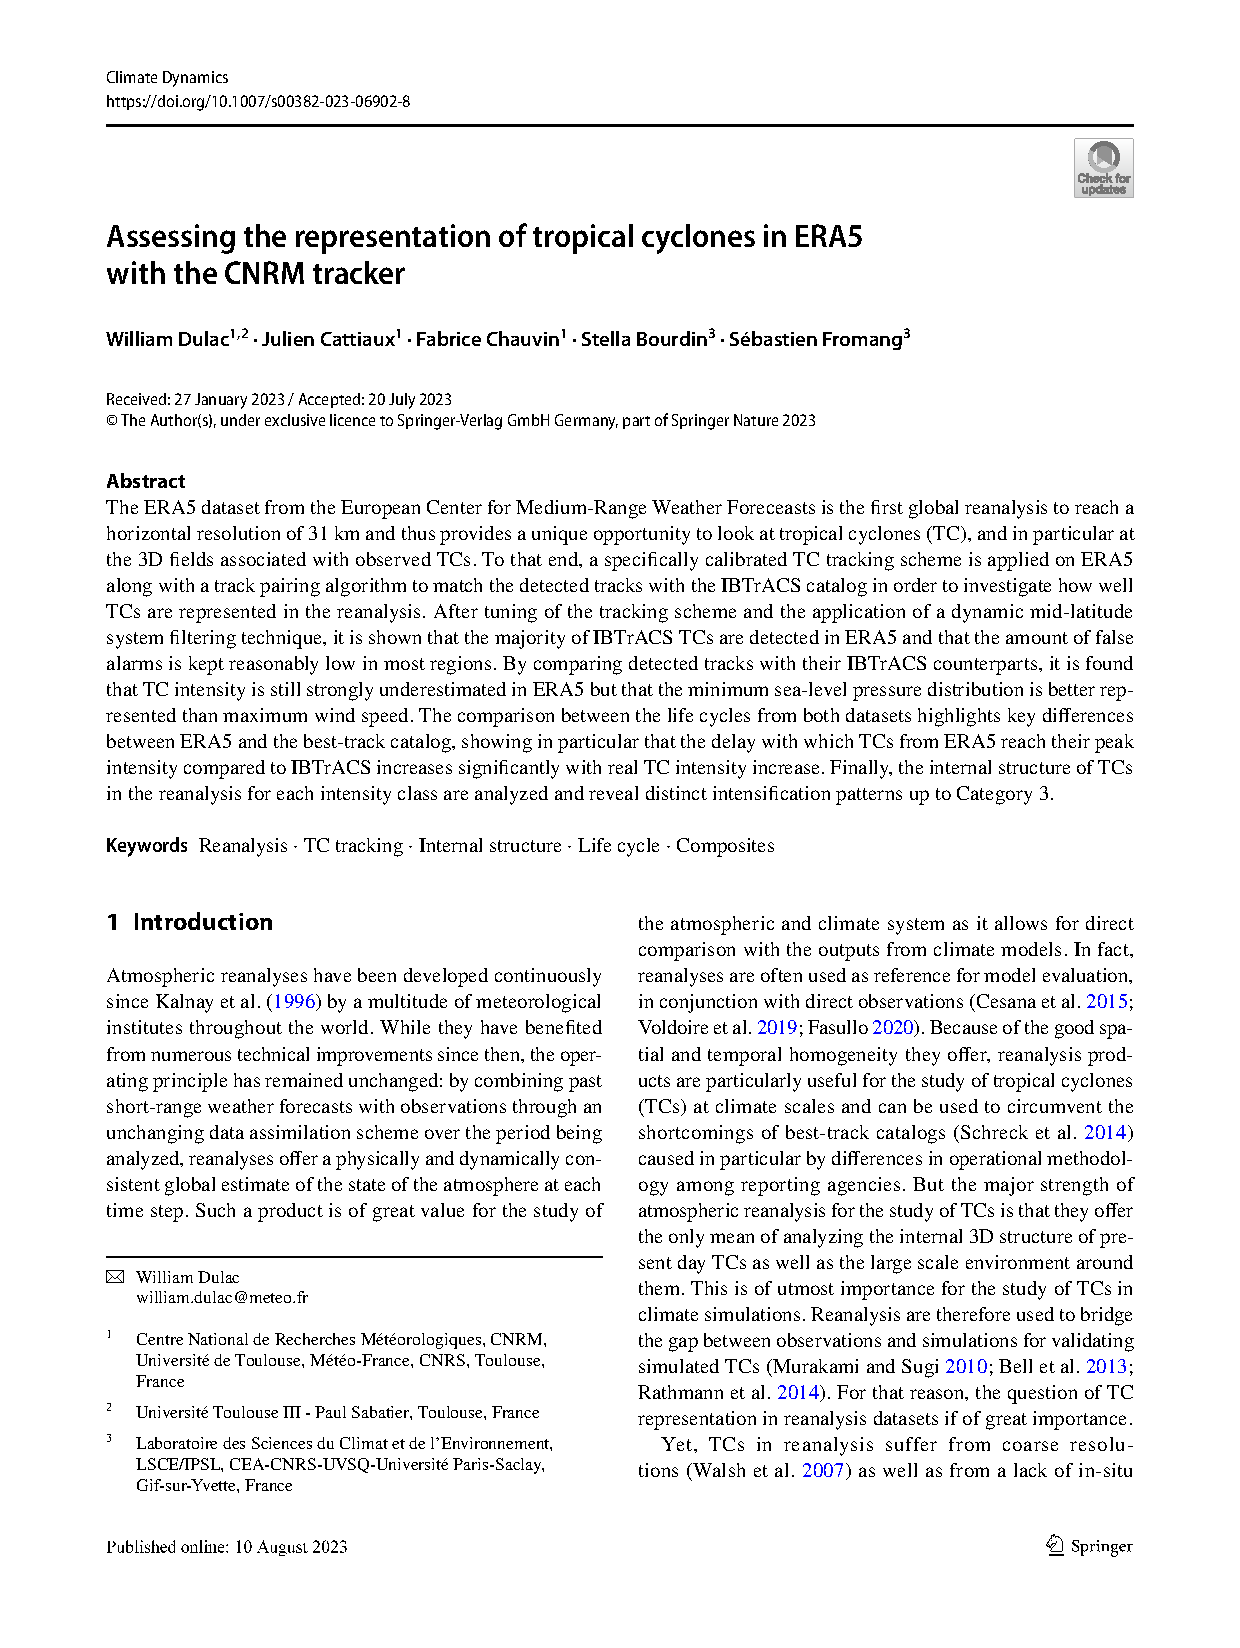
\includepdf[pages=-,pagecommand={\thispagestyle{plain}},offset=5mm 0mm,scale=1,addtotoc=
    {1,subsection,1,Article Climate Dynamics,sec:papier,
     1,subsubsection,2,Introduction,sec:papier_intro,
     2,subsubsection,2,Données et Méthodes,sec:papier_data_methods,
     4,subsubsection,2,Résultats,sec:papier_results,
     10,subsubsection,2,Discussion et conclusion,sec:papier:discussion,
     12,subsubsection,2,Annexe A: Optimisation du traqueur pour ERA5,sec:papier_appendix_A}]{\subfix{../include/dulac2023.pdf}}
%
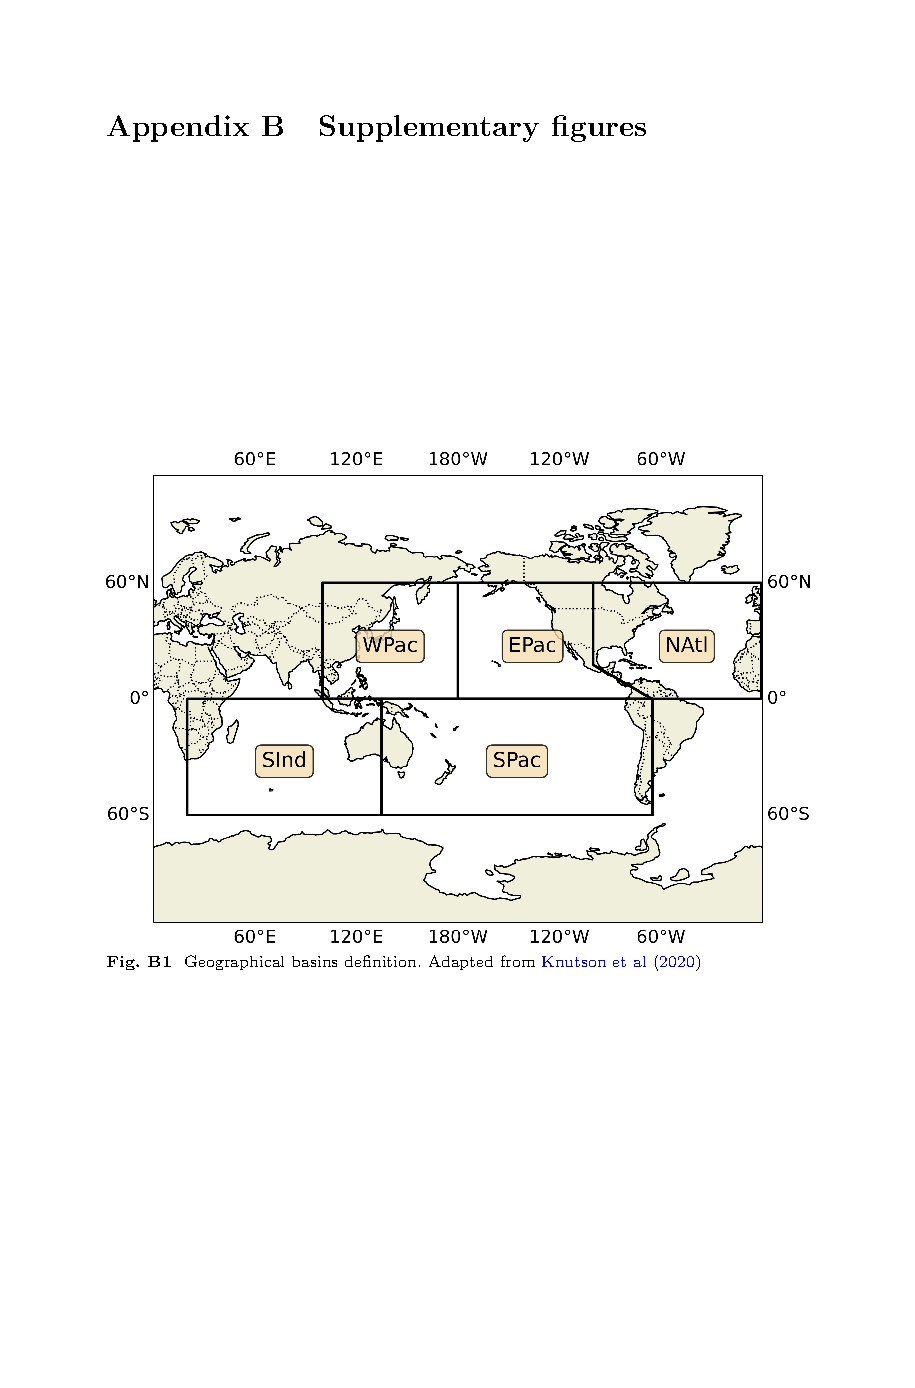
\includepdf[pages=-,pagecommand={\thispagestyle{plain}},offset=5mm 0mm,addtotoc=
{1,subsubsection,2,Annexe B: Figures supplémentaires,sec:papier_appendix_B}]{\subfix{../include/appendix_B_empty.pdf}}

\section{Compléments}\label{sec:complements_papier}

\subsection{Filtrage des systèmes de moyennes latitudes}\label{sec:filtrage_mid_latitudes}

\subsection{Métriques d'évaluation de la similarité des trajectoires}\label{sec:similarité}

\subsubsection*{Introduction}

Les travaux réalisés dans \cite{dulac_assessing_2023} et présentés dans la \cref{sec:papier} font appel aux notions de FAR et POD pour évaluer la performance de
le schéma de détection de TC du CNRM. Le calcul du POD s'appuie sur un algorithme qui associe les trajectoires détectées dans ERA5 à celles présentes dans la
base de données IBTrACS par correspondance spatio-temporelle. Si en moyenne le taux de recouvrement des trajectoires appariés (\textquote{\textit{matched}} dans
\cite{dulac_assessing_2023}) ---~c'est à dire le nombre de points ERA5 situés à moins de \km{300} d'IBTrACS rapporté au nombre d'échéances de la trajectoire
IBTrACS, tel que défini dans la \cref{sec:papier_data_methods}~--- est de \prct{68} (médiane à \prct{71}), il suffit dans l'absolu d'un seul pas de temps
remplissant la condition pour que la trajectoire ERA5 soit appariée à une trajectoire présente dans les observations, et donc pour que la trajectoire détectée
contribue au POD. Ce cas est néanmoins rare puisqu'il concerne en tout et pour tout \num{7} paires de trajectoires ERA5 / IBTrACS, mais on note cependant que
près de \prct{4} de nos trajectoires ERA5 ont un taux de recouvrement inférieur ou égal à \prct{25}. Par ailleurs, le taux de recouvrement des couples de
trajectoires ainsi formés tend à augmenter avec l'intensité des cyclones observés, comme le montre la \cref{fig:coverage_ratio} encadré (a), et qui s'explique
par le fait que les cyclones les plus intenses sont les plus facilement détectables par le traqueur. Cette tendance à de meilleurs recouvrements pour les
cyclones les plus forts n'empêchent pas une certaine dispersion des valeurs. Par exemple \prct{5} des trajectoires appariés à des TC de catégorie \num{3} ont un
taux de recouvrement inférieur ou égal à \prct{31}. Une partie de la variance dans ces scores peut s'expliquer par le fait que le traqueur du CNRM est
susceptible de manquer le début et la fin du cycle de vie des trajectoires observées, en dépit du mécanisme de relaxation des paramètres utilisé dans le schéma
de détection \parencite[][Figure 8]{bourdin_intercomparison_2022}, auquel cas le recouvrement s'en voit mécaniquement réduit. L'autre facteur est que les
trajectoires ERA5 peuvent localement s'éloigner à plus de \km{300} d'IBTrACS. La \cref{fig:coverage_ratio} encadré (b) montre la distribution de la fraction des
points ERA5 situés à plus de \km{300} des observations pour chaque paire de trajectoire et montre qu'en moyenne \prct{5.8} des points détectés par le traqueur
parmi les trajectoires appariés à IBTrACS sont au delà de la limite d'appariement. De plus, \prct{5} des trajectoires détectées dans ERA5 ont une fraction
divergente d'au moins \prct{26}. Par conséquent, la trajectoire détectée dans la réanalyse n'est pas toujours identique à celle du catalogue des best tracks,
soit parce que le traqueur n'en détecte qu'une partie, soit parce que la trajectoire détectée diverge des observations, ou encore par une combinaison quelconque
de ces deux éléments. Enfin, bien que le taux de recouvrement donne une indication sur la similarité des deux trajectoires, il n'apporte pas d'information sur
les variations locales dans la direction de déplacement, ni ne quantifie les cas où la trajectoire ERA5 dépasse celle observée en amont ou en aval, si bien que
ce dernier n'est pas adapté pour évaluer quantitativement la ressemblance entre les trajectoires détectées dans la réanalyse et celles issues des observations.

\begin{figure}[tb]
    \centering
    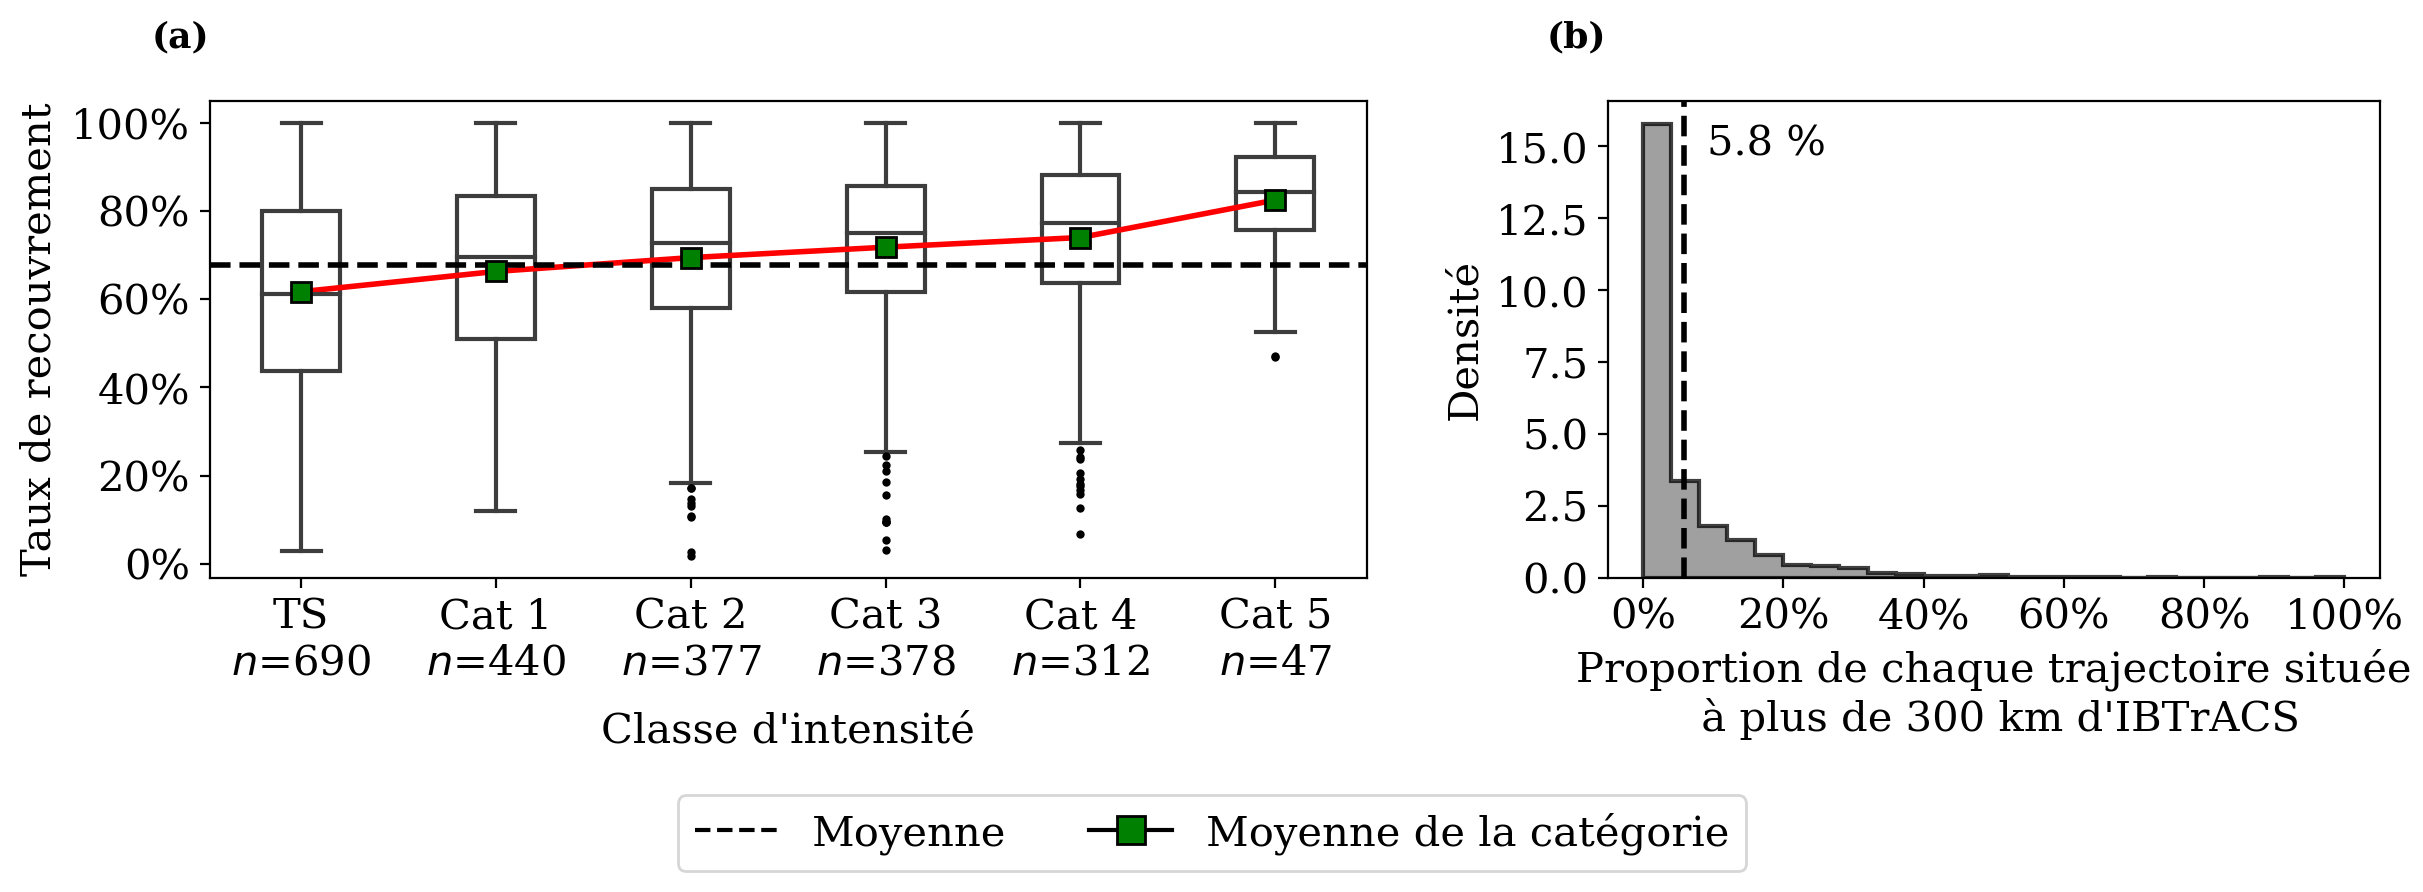
\includegraphics[width=\textwidth]{coverage_ratio_and_missed.png}
    \caption{\textbf{(a)} Distributions des taux de recouvrement des trajectoires appariées entre ERA5 / IBTrACS pour chaque classe d'intensité des TC observés.
    \textbf{(b)} Histogramme de la fraction de points détectés situés à plus de \km{300} d'IBTrACS parmi les trajectoires appariés.}
    \label{fig:coverage_ratio}
\end{figure}

Il existe dans la littérature des algorithmes d'évaluation de la similarité de séries temporelles
\parencite{faloutsos_fast_1994,das_finding_1997,frentzos_indexbased_2007}, mais ces derniers sont plutôt conçus pour des séries uni-dimensionnelles que pour des
trajectoires spatiales car sont souvent basés sur la distance euclidienne qui les sépare. \cite{nakamura_shapebased_2013} proposent une approche basée plutôt
sur la mesure de la similarité de la forme entre deux séries par l'analyse de l'angle formé par les séries, métrique nommée \textit{Angular Metric for Shape
Similarity} (AMSS). Bien que leur approche soit pleinement capable de s'appliquer à des trajectoires spatiales, certaines propriétés de leur métrique ne sont
pas pertinentes (voire pas souhaitables), dans le cas précis des trajectoires de cyclones tropicaux, telles qu'une forte résilience à un décalage temporel entre
les deux séries (pas applicable à des trajectoires appariées entre réanalyse et observations), ainsi qu'une robustesse à des changements isolés de direction.
Ces propriétés rendent par ailleurs leur algorithme très couteux en temps de calcul. Néanmoins, l'aspect novateur derrière les travaux de
\cite{nakamura_shapebased_2013} est repris ici, à savoir la décomposition de la trajectoire en série de vecteurs, détaillée ci-après. Dans cette section, trois
métriques de similarité des trajectoires sont définies et comparées sur le jeu de données issu de \cite{dulac_assessing_2023} et composé des trajectoires
détectées dans la réanalyse ERA5 qui sont appariées à des trajectoires historiques IBTrACS. En particulier, cette analyse vise à déterminer si le réglage des
seuils de détection du traqueur de TC du CNRM dans le but de maximiser le POD ne risque pas de produire des trajectoires peu ressemblantes, du fait de la
formulation de la condition nécessaire et suffisante à l'appariement de deux trajectoires.

\subsubsection*{La similarité angulaire}

\begin{figure}[htbp]
    \centering
    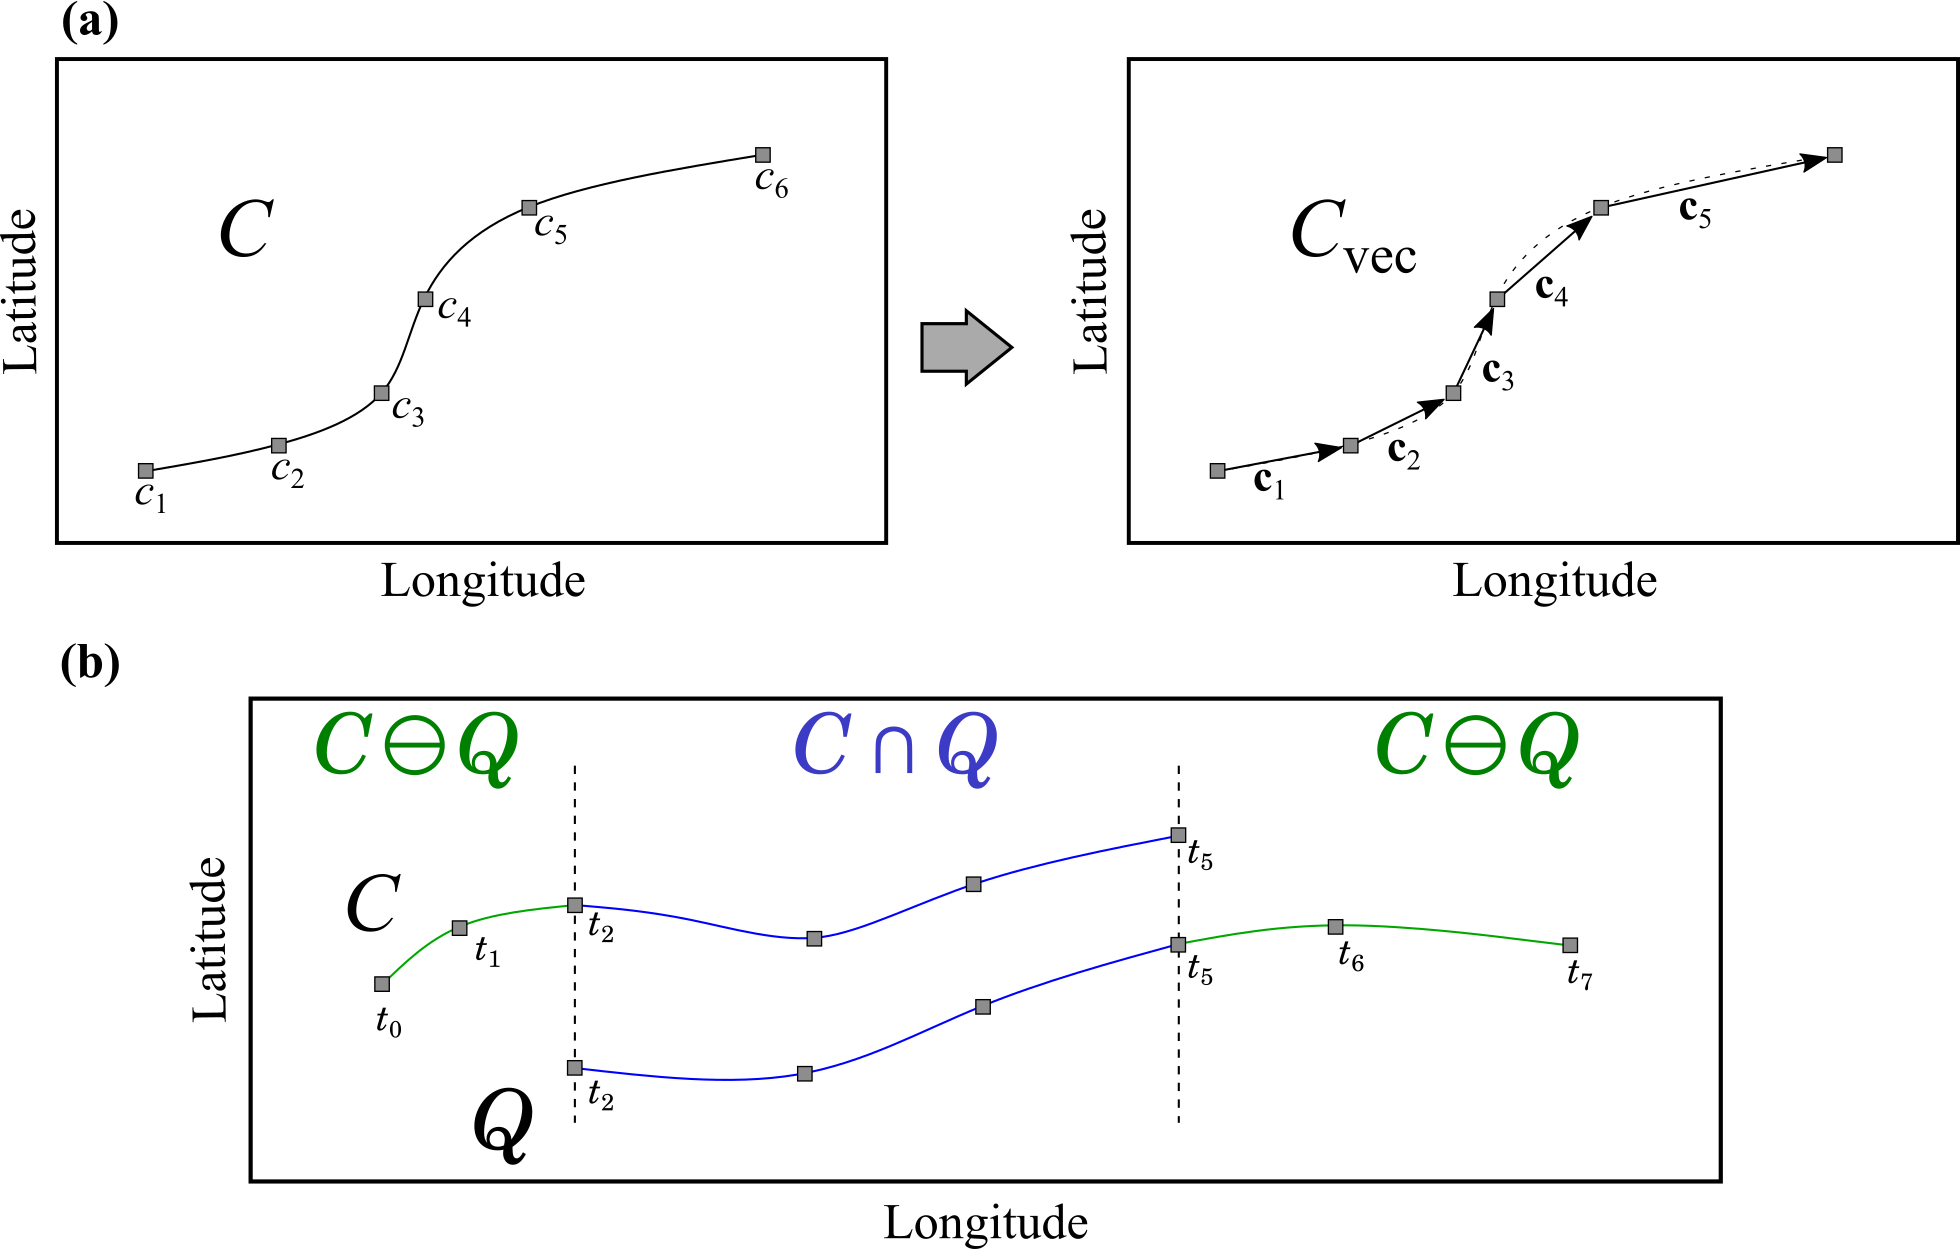
\includegraphics[width=\textwidth]{schema_vec_sequence.png}
    \caption{Représentation schématique de la décomposition d'une trajectoire $C$ en séquence de vecteurs de déplacements relatifs $C_{\text{vec}}$ (a),
    inspirée de \cite{nakamura_shapebased_2013}. Représentation visuelle de $C \cap Q$ et de $C \ominus Q$ (b). Dans cet exemple, $N_\cap = N_\ominus = 4$.}
    \label{fig:schema_trajectoires}
\end{figure}

Une trajectoire de cyclone tropical est une série temporelle composée des positions successives du système et accompagnées de diverses informations permettant
la caractérisation du système, telles que le vent maximum ou la pression centrale. Pour pouvoir évaluer la similarité entre deux trajectoires, on considère non
pas les positions discrètes du système, mais plutôt la série de vecteurs décrivant le déplacement relatif entre chaque position successive.

Reprenant le formalise de \cite{nakamura_shapebased_2013} ; soit $C$ une trajectoire de TC composée de $M+1$ pas de temps et définie par ses positions
$p_{1...M+1}$ sur une grille géo-référencée et aux temps $t_{1...M+1}$ :
%
\begin{align*}
    C &= ((p_1, t_1), (p_2, t_2), \ldots, (p_{M+1}, t_{M+1}))\\
      &= (c_1, c_2, \ldots, c_{M+1})
\end{align*}
%
Alors la série des vecteurs de déplacement équivalente $C_{\text{vec}}$ est donnée par :
\begin{align*}
    C_{\text{vec}} &= ((c_2 - c_1), (c_3 - c_2), \ldots, (c_{M+1} - c_M))\\
            &= (\mathbf{c}_1, \mathbf{c}_2, \ldots, \mathbf{c}_M)
\end{align*}
%
tel qu'illustré par la \cref{fig:schema_trajectoires}, encadré (a). Soit $Q_{\text{vec}}$ la série des vecteurs de déplacements d'une seconde trajectoire composée de
$M^\prime$ vecteurs. L'angle $\theta$ entre deux vecteurs individuels $\mathbf{c}_i$ et $\mathbf{q}_j$ issus respectivement de $C_{\text{vec}}$ et
$Q_{\text{vec}}$, et où $i$ et $j$ correspondent au même temps $t$ est donné par le produit scalaire des deux vecteurs. $\cos \theta$ est aussi appelé
similarité cosinus et est noté $S_C$ :
%
\begin{equation*}
    S_C(\mathbf{c}_i, \mathbf{q}_j) = \cos \theta = \frac{\mathbf{c}_i \cdot \mathbf{q}_j}{\lVert \mathbf{c}_i \rVert \lVert \mathbf{q}_j \rVert} \in [-1; 1] 
\end{equation*}
%
Ainsi la similarité cosinus caractérise l'angle formé par les vecteurs de déplacement issus de deux trajectoires à un instant donné. On peut ensuite définir la
distance angulaire, ou angle normalisé, qui est une distance formelle au sens où l'inégalité de Cauchy-Schwartz est respectée, par :
%
\begin{equation*}
    D_\theta = \frac{\theta}{\pi}
\end{equation*}
%
Et son complément, appelé similarité angulaire par :
%
\begin{equation*}
    S_\theta = 1 - D_\theta = 1 - \frac{\theta}{\pi} \in [0; 1]
\end{equation*}
%
C'est cette dernière distance $S_\theta$ qui est utilisée dans cette analyse. De cette façon, la plus faible similarité entre deux vecteurs est atteinte
lorsqu'ils sont parallèles mais de sens opposés, tandis que la similarité est maximale si deux vecteurs parallèles sont de même sens.

\subsubsection*{Métriques de similarité intégrée}\label{sec:definition_MAS}

Avant de définir les trois métriques, il est important de distinguer trois membres dans un couple de trajectoires appariées. En effet, la similarité angulaire
$S_\theta$ est définie ci-dessus pour deux vecteurs correspondants aux déplacements entre deux positions successives, pour deux trajectoires prises au même
temps $t$. Or, il est admis qu'un des deux vecteurs peut ne pas exister à cet instant si le schéma de détection n'a pas capturé l'entièreté de la trajectoire ou
au contraire si la trajectoire détectée est plus longue que celle observée, aussi bien en amont qu'en aval. On appelle donc l'intersection des trajectoires $C
\cap Q$ le sous-ensemble des pas de temps dans lequel les deux trajectoires co-existent et où chaque paire de points correspond au même temps $t$.
Réciproquement, l'union $C \cup Q$ contient l'entièreté des échéances consistuant le couple de trajectoires. Enfin, la différence symétrique des deux
trajectoires $C \ominus Q$ contient les pas de temps pour lesquels une seule trajectoire existe à la fois. La \cref{fig:schema_trajectoires} encadré (b)
illustre schématiquement ces notions.

En première approche, on peut définir la similarité intégrée entre deux trajectoires $C$ et $Q$ comme la moyenne de la similarité angulaire $S_\theta$ sur $C
\cap Q$, notée $\bar{S_\theta}^\cap$ (\textit{Mean Angular Similarity}, MAS):
%
\begin{equation}
    \bar{S_\theta}^\cap = \frac{1}{N_\cap} \sum_{i=1}^{N_\cap} S_\theta (\mathbf{c}_i, \mathbf{q}_i) \tag*{MAS$^\cap$}
\end{equation}
%
Cette première métrique de similarité se concentre donc sur les échéances où les deux trajectoires coexistent, les échéances non-détectées ainsi que celles en
trop par rapport aux observations n'étant pas compatiblisées.

Comme variante, on définit aussi le MAS sur l'union des deux trajectoires en remplaçant le dénominateur par $N_\cup = N_\cap + N_\ominus$. Cela revient
à considérer que les echéances sur $C \ominus Q$ ont une similarité angulaire artificiellement fixée à \num{0} :
%
\begin{equation}
    \bar{S_\theta}^\cup = \frac{1}{N_\cup} \sum_{i=1}^{N_\cap} S_\theta (\mathbf{c}_i, \mathbf{q}_i) \tag*{MAS$^\cup$}
\end{equation}
%
Ainsi, cette seconde métrique de similarité considère l'entièreté des deux trajectoires constituant le couple ERA5 / IBTrACS dans le calcul de la similarité, au
risque d'être très punitif si $N_\ominus \neq 0$.

On définit enfin une troisième métrique de similarité, pensée comme un hybride entre MAS$^\cap$ et MAS$^\cup$ dans sa prise en compte des échéances sur $C
\ominus Q$. Cette dernière métrique, nommée wMAS (\textit{weighted}), considère toujours comme nulle la similarité sur $C \ominus Q$, mais introduit deux
coefficients $w_1$ et $w_2$, en concurrence l'un contre l'autre, qui vont peser différemment sur $C \cap Q$ et $C \ominus Q$ respectivement, et qui s'expriment
comme fonction de $\bar{S_\theta}^\cap$ :
%
\begin{equation*}
\text{wMAS} = \frac{ w_1\sum_{i=1}^{N_\cap} S_{\theta}(\mathbf{c}_i, \mathbf{q}_i) }{ w_1 N_\cap + w_2 N_\ominus}\quad\quad \tag*{wMAS}
    \begin{cases}
        w_1 = a + \bar{S_\theta}^\cap \. , \;\; a \geq 0 \\
        w_2 = b - \bar{S_\theta}^\cap \. , \;\; b \geq 1 \\
    \end{cases}
\end{equation*}
%
Le wMAS vise à fournir une valeur quantitative du ressenti qualitatif de la similarité d'une paire de trajectoires, en ce sens que le plus la similarité moyenne
sur $C \cap Q$ est élevée, le moins la taille de $C \ominus Q$ a d'importance dans la similarité totale, et réciproquement. Le wMAS traduit donc l'idée
subjective que la similarité sur l'intersection des trajectoires peut compenser partiellement la différence de taille entre une trajectoire détectée associée à
une trajectoire observée. Le degré d'intensité de cette compensation (ou respectivement de pénalisation) peut être ajusté via les paramètres $a$ et $b$. Ici ces
paramètres sont empiriquement fixés à $a=1$ et $b=2$. Par construction, on a :
%
\begin{equation*}
    \text{MAS}^\cap \geq \text{wMAS} \geq \text{MAS}^\cup
\end{equation*}

\subsubsection*{Application}

La \cref{fig:MAS_Ndiff} présente la similarité des trajectoires appariées entre ERA5 et IBTrACS en fonction du nombre d'échéances non partagées entre elles,
c'est à dire pour les temps où une seule des deux est définie, $N_\ominus$.
%
\begin{figure}[htpb]
    \centering
    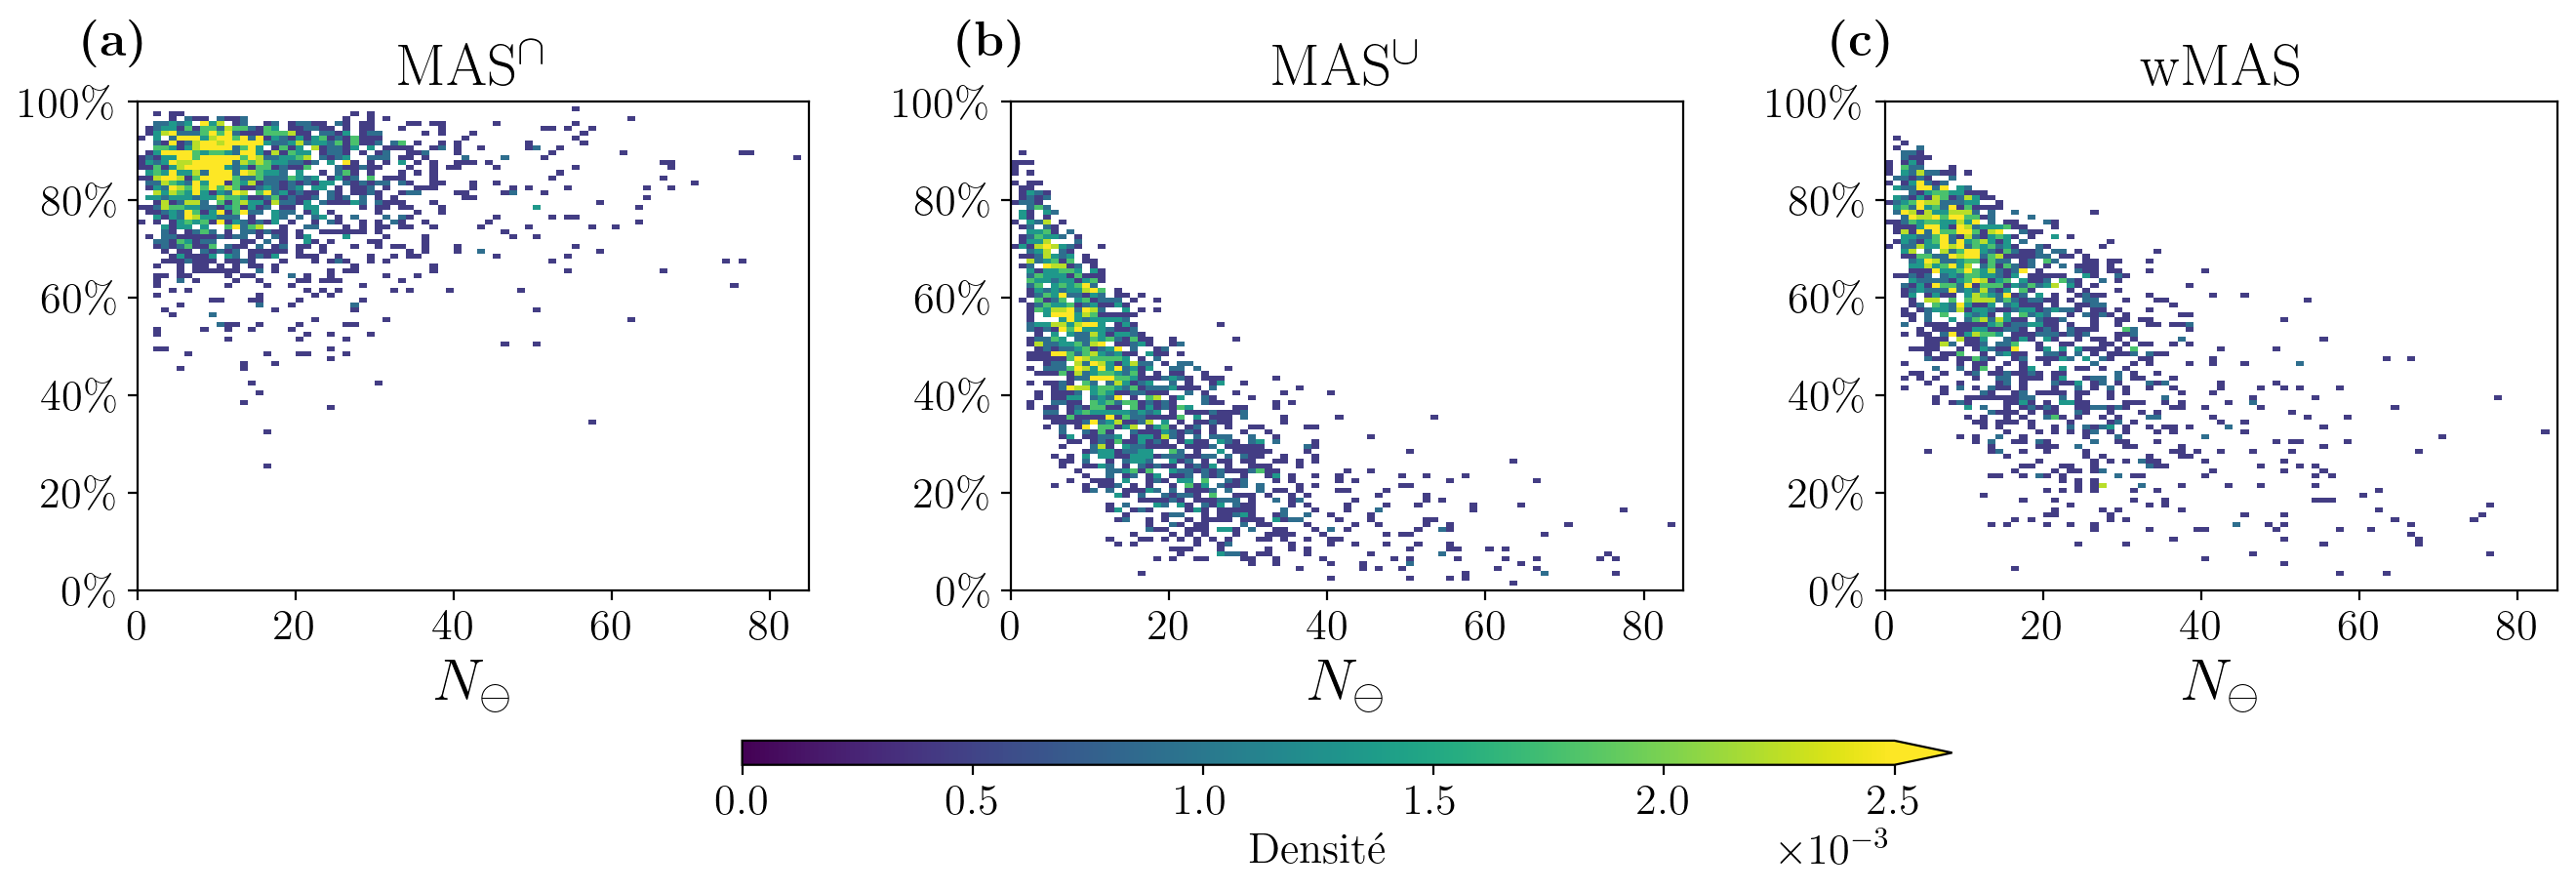
\includegraphics[width=\textwidth]{MAS_vs_Ndiff.png}
    \caption{Caractérisation de la relation entre la similarité des trajectoires en pourcentage et le nombre $N_\ominus$ d'échéances \num{6}-horaires contenu
    dans $C \ominus Q$, pour les trois métriques MAS$^\cap$, MAS$^\cup$ et wMAS de gauche à droite respectivement (a,b et c), évaluées sur \num{2244} paires de
    trajectoires ERA5 / IBTrACS.}
    \label{fig:MAS_Ndiff}
\end{figure}
%
De par sa définition, le MAS$^\cap$ ne dépend que des vecteurs de déplacement sur l'intersection des trajectoires, si bien qu'aucune relation avec $N_\ominus$
ne se dégage. L'encadré (a) met également en évidence une grande similarité angulaire moyenne, avec un MAS$^\cap$ moyen et médian à \prct{83} et \prct{85},
respectivement. La dispersion de ces scores est également très faible, avec un écart type à \prct{9}. Toutefois, la distribution jointe de MAS$^\cap$ montre
également le défaut de cette métrique, puisqu'une similarité évaluée à plus de \prct{80} lorsque $N_\ominus$ est large (jusqu'à $10 N_\cap$) pose question sur
le sens de cette mesure. C'est en réponse à ce constat que le MAS$^\cup$ a été défini, dont la distribution jointe avec $N_\ominus$ est présentée sur la
\cref{fig:MAS_Ndiff}, encadré (b). Pour cette seconde métrique, les scores de similarité sont d'une part diminués, et également largement dispersés. Le
MAS$^\cup$ présente en effet une moyenne et une médiane tous deux à \prct{42} ---~soit près de deux fois moins qu'avec MAS$^\cap$~--- tandis que l'écart-type
est de \prct{18}. En outre, cette métrique présente une relation très marquée avec $N_\ominus$, quasi-linéaire jusqu'à environ $N_\ominus = 20$, au delà de quoi
la similarité apparaît comme légèrement moins sensible à la différence de taille. La différence entre MAS$^\cap$ et MAS$^\cup$ est particulièrement prononcée,
et l'impact de $N_\ominus$ sur MAS$^\cup$ est très fort, à tel point que le problème inverse à celui de MAS$^\cap$ peut se poser, à savoir que la
comptabilisation des échéances sur $C \ominus Q$ avec le même poids que celles sur $C \cap Q$ peut parfois s'avérer très punitive, comme illustré sur les trois
exemples de la \cref{fig:exemple_MAS}. Le wMAS (\cref{fig:MAS_Ndiff} encadré c) vise donc à compenser cette propriété du MAS$^\cup$ via ses coefficients de
pondération qui modifient la contribution de $C \cap Q$ et de $C \ominus Q$ en fonction de la similarité moyenne obtenue sur l'intersection. La distribution du
wMAS est intermédiaire entre MAS$^\cap$ et MAS$^\cup$, avec \prct{59} en moyenne et \prct{62} en valeur médiane. Si on distingue toujours une relation linéaire
entre wMAS et $N_\ominus$, la dispersion des valeurs de $N_\ominus$ autour du score moyen est plus élevée que dans le cas de MAS$^\cup$, indiquant que le wMAS
parvient en effet à compenser des valeurs larges de $N_\ominus$ lorsque $\bar{S_\theta}^\cap$ est élevé. Les exemples de la \cref{fig:exemple_MAS} illustrent ce
point. Ce faisant, le wMAS perd néanmoins en interprétabilité.

\begin{figure}[htbp]
    \centering
    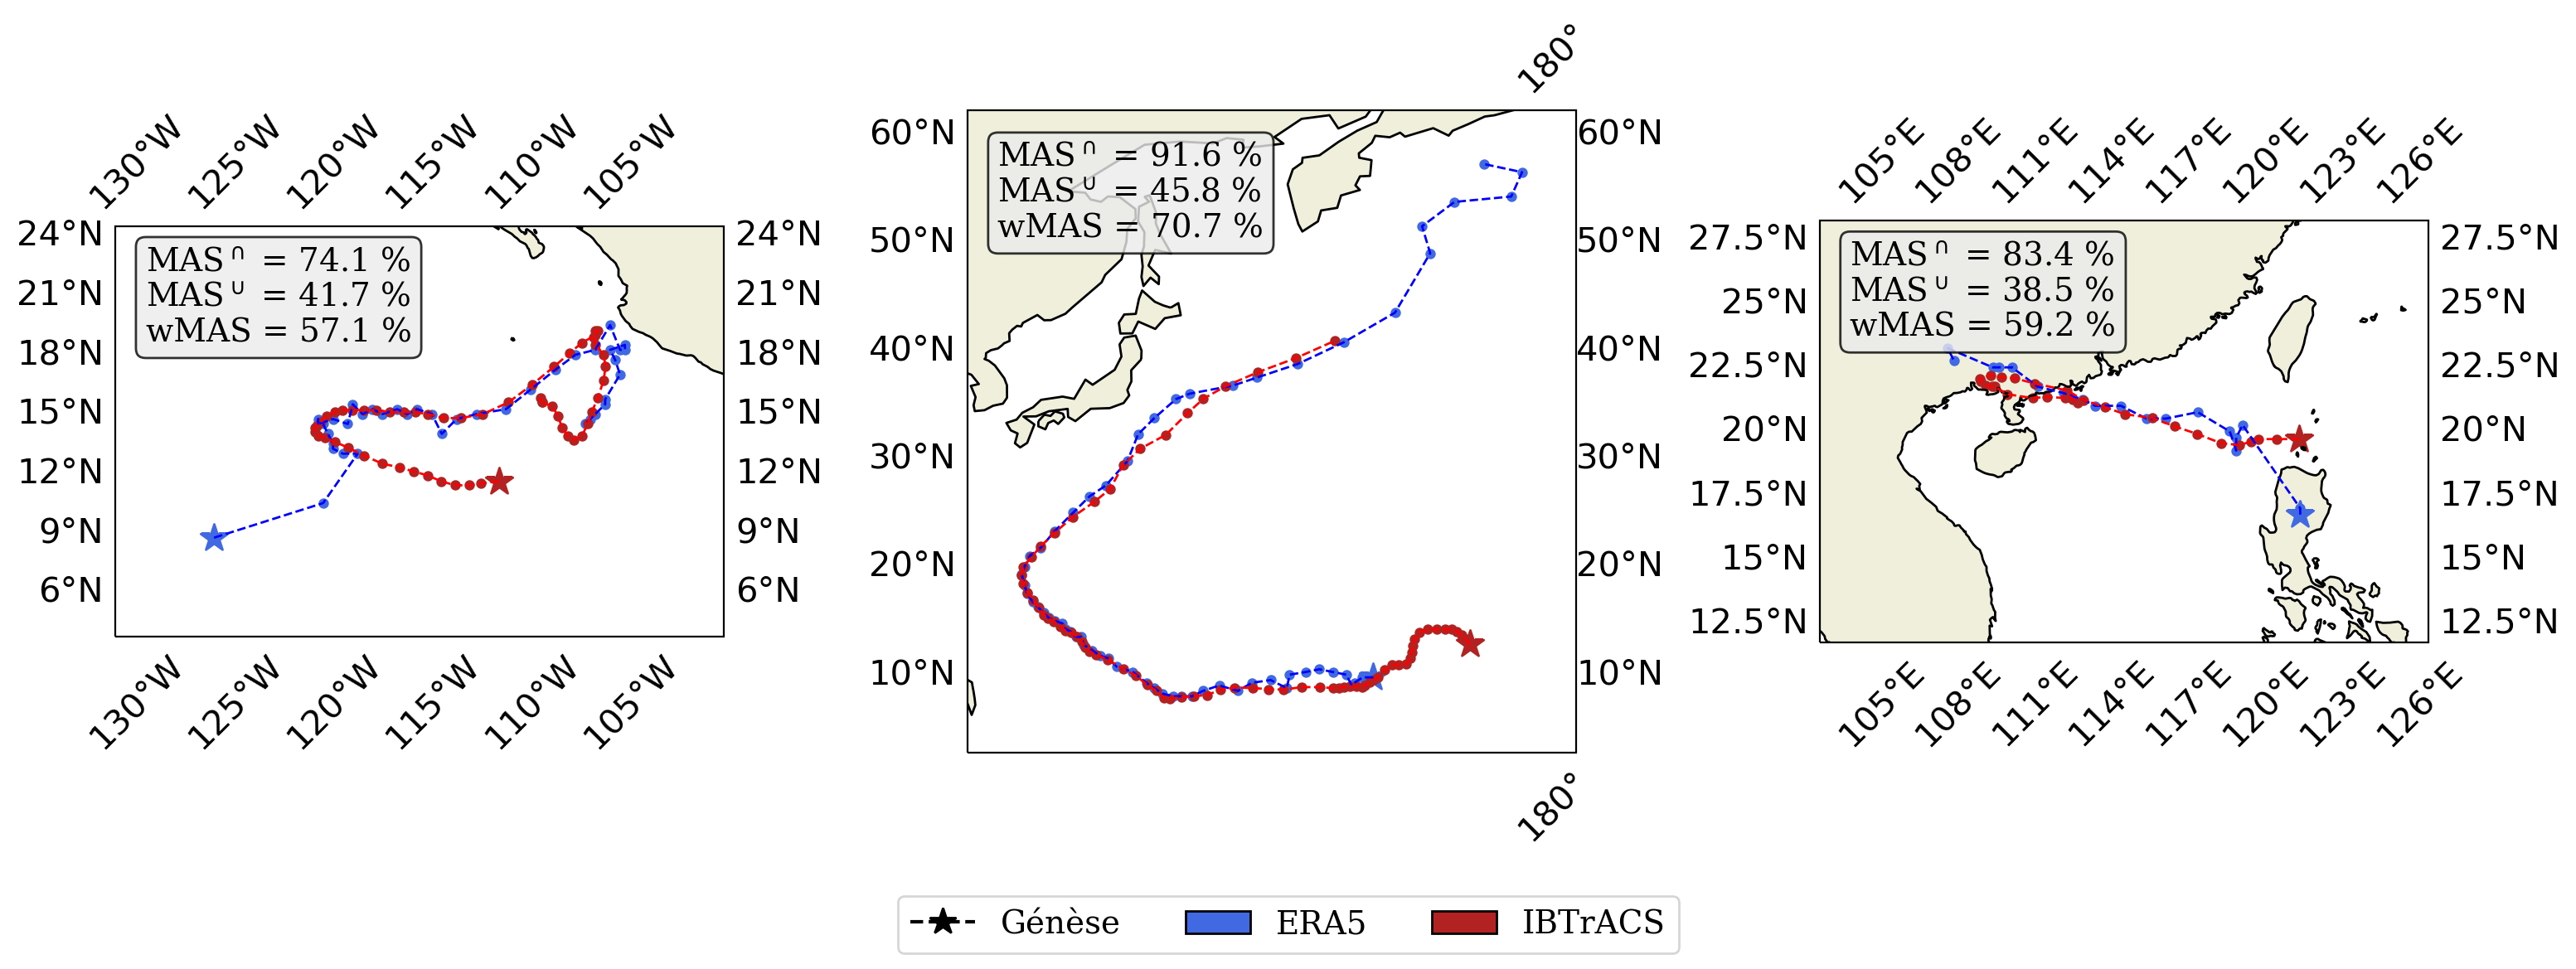
\includegraphics[width=\textwidth]{exemple_MAS_3_tracks.png}
    \caption{Exemple de trois paires de trajectoires sélectionnées parmi les \num{2244}, avec leurs scores de similarité pour chacune des trois métriques
    indiqués dans l'encadré en haut à gauche.}
    \label{fig:exemple_MAS}
\end{figure}

Pour déterminer si l'ajustement des paramètres de détection dont a fait l'objet le traqueur dans le but de maximiser la probabilité de détection a affecté la
similarité des trajectoires, on calcule les valeurs des trois métriques de MAS pour les couples de trajectoires ERA5 / IBTrACS obtenus avant l'optimisation afin
de les comparer aux similarités que les trajectoires actuelles présentent avec ces mêmes trajectoires IBTrACS. Les tracjectoires ERA5 dites
\textquote{non-optimisées} et prises comme référence ici ont été obtenues avec les seuils \textbf{VOR}~$=$~\SI{5e-5}{\per\second}, \textbf{RES}~$=$~\ms{15},
\textbf{TANOM}~$=$~\SI{1}{\kelvin}, \textbf{PT}~$=$~\SI{-2}{\kelvin} et \textbf{PW}~$=$~\ms{5}. Ces valeurs seuils se distinguent de celles utilisées dans
\cite{dulac_assessing_2023} et \cite{bourdin_intercomparison_2022} par la vorticité (respectivement \SI{15e-5}{\per\second}), le seuil de vent (respectivement
\ms{5}) ainsi que le profil vertical de température (respectivement \SI{-1}{\kelvin}). Le paramètre de relaxation est maintenu à \SI{25e-5}{\per\second} entre
les deux jeux de données. La solution non-optimisée présente un POD moyen sur les cinq bassins d'intérêt diminué de plus de \num{10} points de pourcentage,
l'impact le plus prononcé étant sur les bassins NAtl et EPac. Cette diminution du POD se traduit par un déficit de \num{465} couples ERA5 / IBTrACS par rapport
aux trajectoires optimisées, puisque \num{1779} trajectoires ERA5 sont appariées avec les trajectoires de référence. Parmi ces paires de trajectoires,
\num{1649} d'entre elles partagent la même composante IBTrACS, indiquant que \num{130} paires sont manquantes dans les trajectoires dites
\textquote{optimisées}. Cette perte peut s'expliquer par le coût non-négligeable en POD du filtre de systèmes de moyennes latitudes utilisé dans
\cite{dulac_assessing_2023}, filtre non appliqué sur les trajectoires de référence. En effet, le schéma de détection optimisé consiste essentiellement en un
relâchement des contraintes définissant un cyclone tropical, conduisant à un plus grand nombre de systèmes détectés et appariés, notamment des systèmes peu
intenses qui parfois ne présentent pas un cœur chaud suffisamment marqué selon le paramètre $V_U^T$ de \cite{hart_cyclone_2003} sur lequel est fondé le filtre.
Il reste donc \num{1649} cyclones observés dans IBTrACS pour lesquels nous disposons de deux trajectoires ERA5 issues de paramètres de détection différents.
On compare alors la similarité de chacune d'elles évaluée sur le cyclone observé, et pour les trois métriques de similarité présentées précédemment. La première
ligne de la \cref{fig:delta_MAS} présente les distributions de ces changements par rapport aux trajectoires issues du schéma de détection non-optimisé.

\begin{figure}[htb]
    \centering
    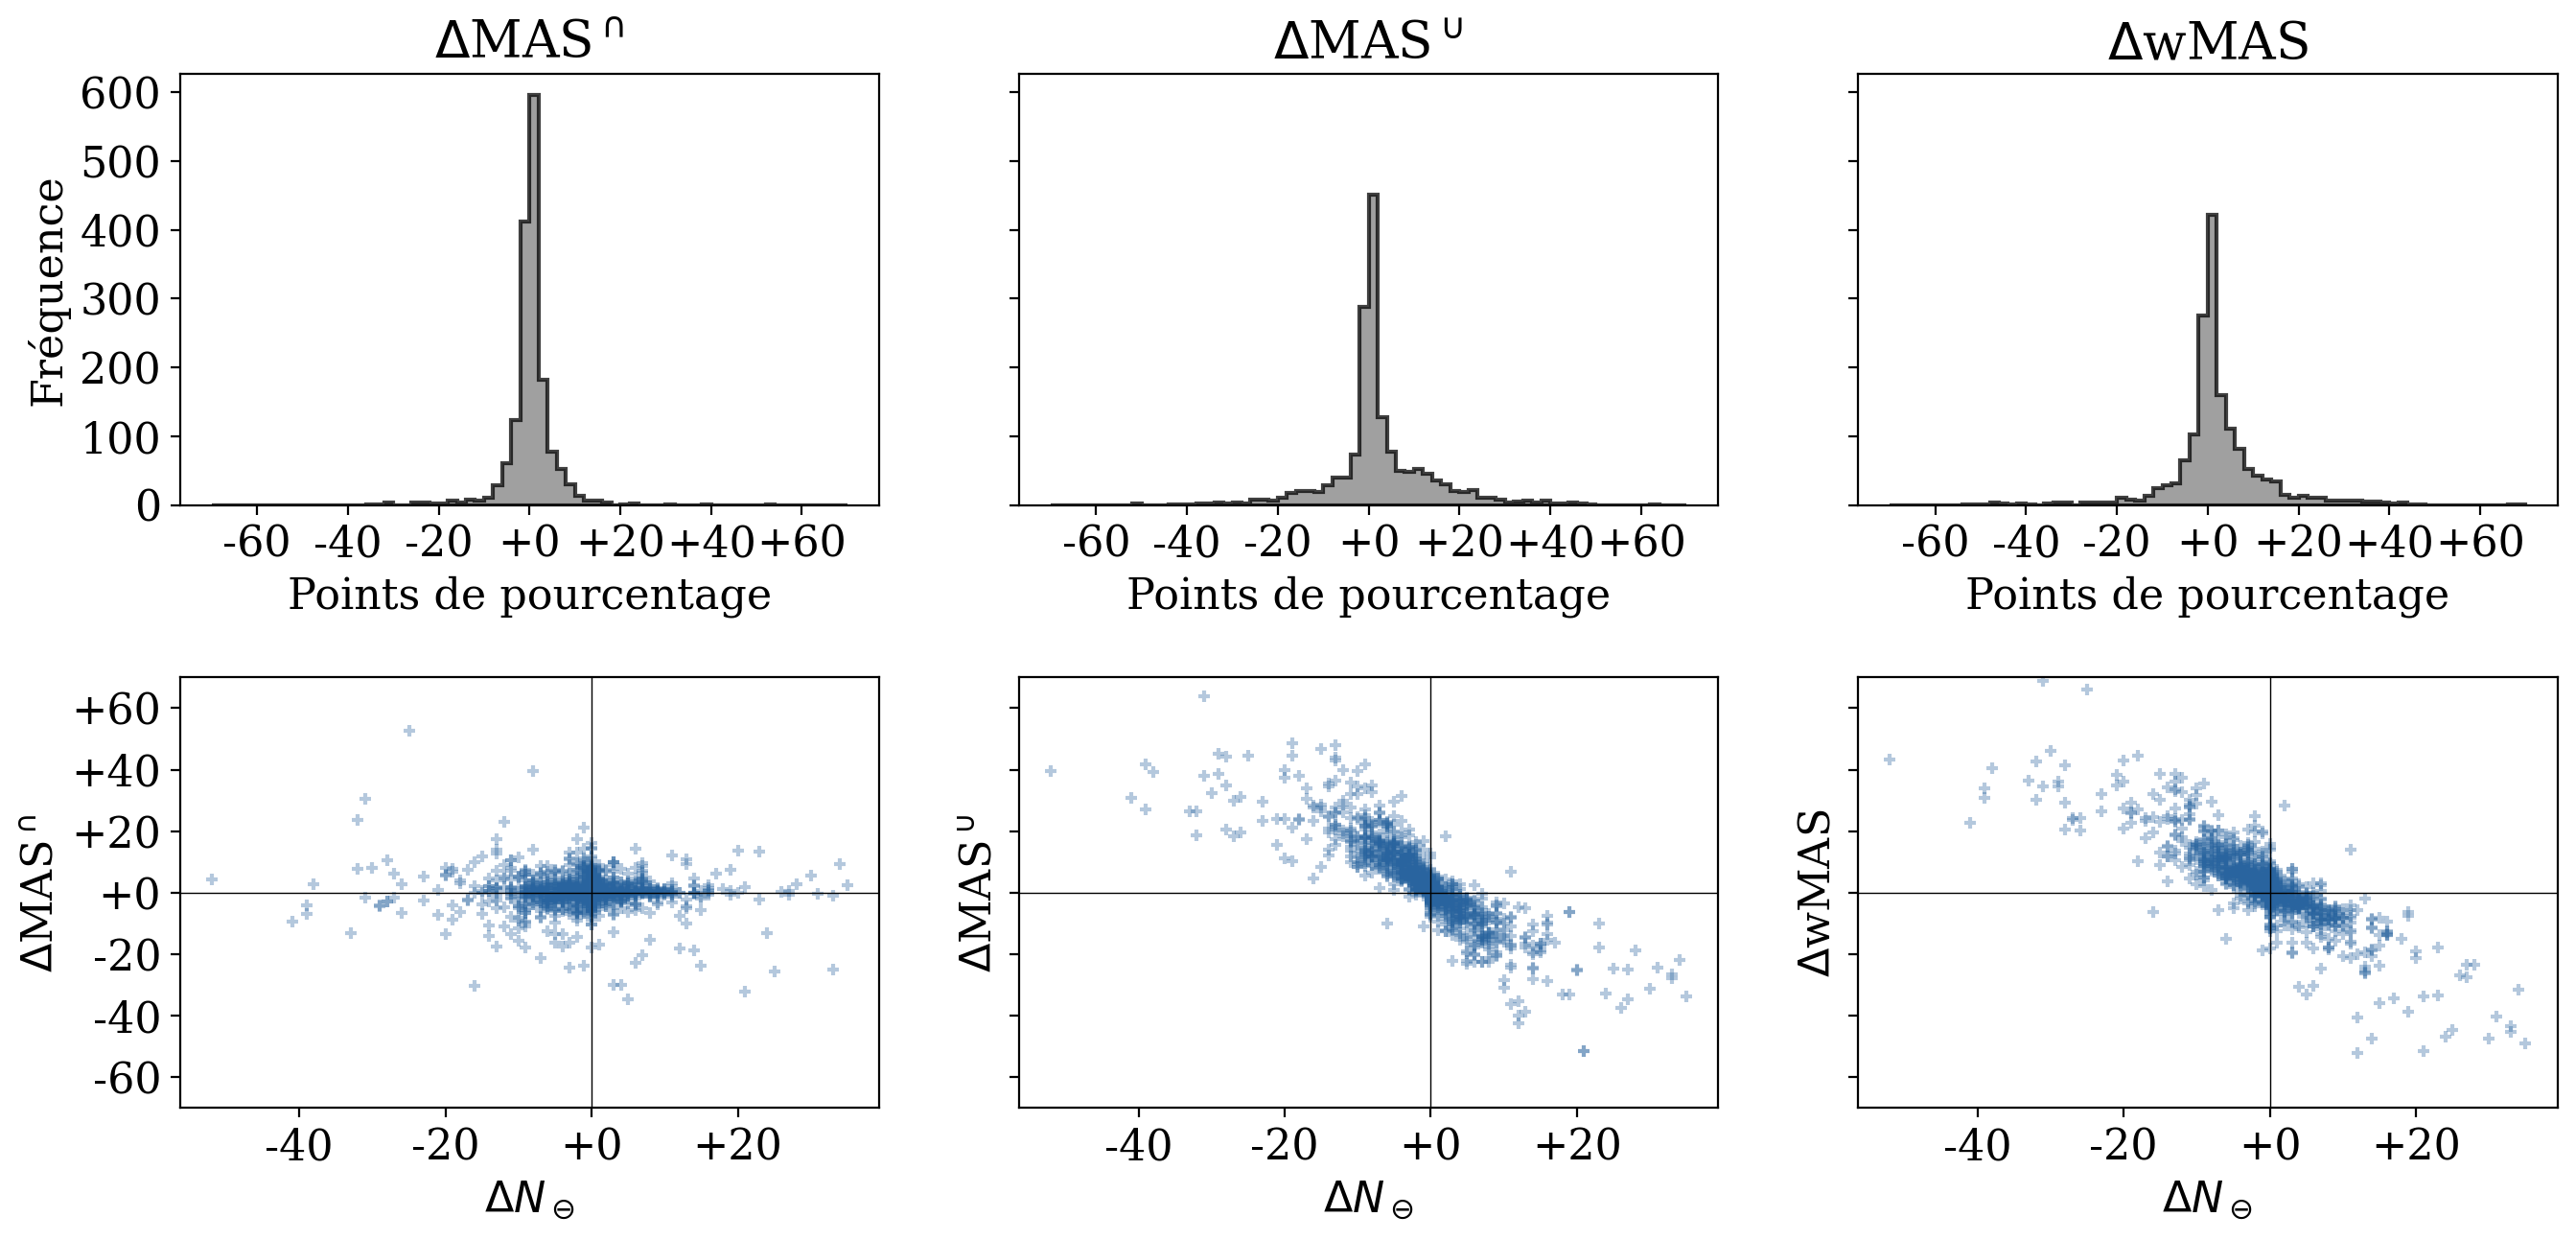
\includegraphics[width=\textwidth]{delta_MAS.png}
    \caption{Distributions du changement dans la similarité des couples de trajectoires ERA5 / IBTrACS (première ligne), par rapport au schéma de détection
    non-optimisé, et pour chacune des trois métriques de similarité (colonnes). Bins de \num{-70} points à \num{70} points avec une largeur de \num{2}
    points. Changement dans la similarité des couples de trajectoires en fonction du changement dans le nombre d'échéances $N_\ominus$ (seconde ligne).}
    \label{fig:delta_MAS}
\end{figure}

Les trois distributions mettent en avant des changements de similarité pour l'essentiel centrés autour de \num{0}. En particulier, la distribution de $\Delta
\text{MAS}^\cap$ présente une moyenne à $+$\num{0.3} points de pourcentage (p.p), et une médiane à $+$\num{0.14} p.p. Si cette moyenne apparaît comme
significativement différente de \num{0} avec test à \prct{95} (valeur-p $=$ \num{0.008}), ce changement est néanmoins insignifiant et peut probablement
s'expliquer par le fait que $N_\cap$ tend à augmenter avec le schéma optimisé ($+$\num{1.9} pas de temps en moyenne), si bien que la similarité angulaire
moyennée sur $C \cap Q$ devient moins sensible aux incohérences locales entre les deux trajectoires. Les deux métriques prenant en considération les échéances
sur $C \ominus Q$ présentent quant à elles une tendance plus claire, bien que toujours faible, vers une amélioration de la similarité, et plus prononcée dans le
cas de MAS$^\cup$ que pour le wMAS. Ces deux distributions indiquent respectivement une moyenne à $+$\num{2.4} p.p et $+$\num{2.05} p.p. Cette évolution est
largement liée au changement de $N_\ominus$ ($-$\num{0.8} pas de temps en moyenne), avec une relation linéaire évidente avec $\Delta N_\ominus$. Un ajustement
linéaire des deux métriques avec $\Delta N_\ominus$ permet d'expliquer \prct{74} de la variance dans le cas de MAS$^\cup$ et \prct{72} dans le cas de wMAS. Mais
cela ne signifie pas pour autant que l'augmentation constatée dans ces deux métriques n'est qu'un artefact. En effet, rappelons que $N_\ominus$ mesure la
différence dans la temporalité des deux trajectoires, si bien que $\Delta N_\ominus < 0$ pour une même trajectoire IBTrACS indique que la trajectoire ERA5 issue
du schéma optimisé présente un début et/ou une fin plus proche de la trajectoire observée. Ainsi, une diminution de $N_\ominus$ avec un MAS$^\cap$ inchangé
constitue en soi une amélioration de la ressemblance des trajectoires. Par ailleurs, il est intéressant de constater sur la seconde ligne de la
\cref{fig:delta_MAS} que, pour les trois métriques considérées, les distributions des changements dans la similarité pour les cas où $\Delta N_\ominus = 0$ sont
faiblement décentrées du côté positif. Précisions toutefois que $\Delta N_\ominus =0$ ne signifie pas nécessairement que les deux trajectoires ERA5 partagent la
même temporalité. Pour s'en convaincre, il suffit de considérer une trajectoire ERA5 qui, dans un jeu de données, ne détecterait pas la dernière échéance de la
trajectoire observée, tandis que la trajectoire équivalente dans le second jeu de données en détecterait une de trop. Une telle situation serait caractérisée
par $\Delta N_\ominus = 0$ et $\Delta N_\cap = +1$. Pour déterminer le changement moyen pour les cas où les deux trajectoires ERA5 sont définies sur exactement
les mêmes dates, il faut donc considérer $\Delta N_\ominus = 0$ et $\Delta N_\cap$ = 0, ce qui correspond à \num{691} cas (\num{721} cas pour la condition
$\Delta N_\ominus = 0$ seule). Le changement moyen de similarité lorsque ces deux conditions sont réunies vaut $+$\num{0.57} p.p, $+$\num{0.34} p.p et
$+$\num{0.54} p.p pour MAS$^\cap$, MAS$^\cup$ et wMAS respectivement. Il semble par conséquent que l'optimisation du schéma de détection de cyclones tropicaux
dans le but de maximiser la probabilité de détection dans ERA5 par rapport à IBTrACS a pu, toutes choses égales par ailleurs, très légèrement améliorer la
similarité des trajectoires détectées avec celles observées, selon la définition de la similarité utilisée ici.

\subsubsection*{Discussion}

En définitive, trois métriques de similarité des trajectoires, toutes basées sur la similarité angulaire $S_\theta$ définie entre deux vecteurs de déplacement
relatif, mais se distinguant par leur prise en charge (ou l'absence) des pas de temps pour lesquels une seule des deux trajectoires existe, sont définis ou
comparés. Étant donné que la similarité de deux trajectoires comporte une part importante de subjectivité, il n'est pas possible de conclure sur les
performances de chacune. Le choix de la métrique dépend en effet de l'usage qui lui est destinée. Le MAS$^\cap$ ne considère que les échéances pour lesquelles
les deux trajectoires coexistent, et peut donc indiquer un excellent score pour des trajectoires pourtant extrêmement différentes. Le MAS$^\cup$ suit la
démarche inverse de compter comme nulle la similarité angulaire sur les échéances où une seule trajectoire existe, si bien qu'une faible différence dans la
taille des trajectoires peut conduire à un score sensiblement diminué. Le wMAS quant à lui, vise à accomplir la tâche pourtant impossible de quantifier avec une
métrique objective une impression subjective de similarité. Si cette approche est par nature vouée à l'échec, le wMAS remplit néanmoins parfaitement son rôle
consistant à nuancer le MAS$^\cup$, se situant ainsi entre les deux autres, et accomplit cela en pondérant les similarités nulles sur $C \ominus Q$ en fonction des
performances sur $C \cap Q$, au détriment de l'interprétabilité de la mesure. Cette caractéristique commune aux trois métriques d'être basées sur une valeur moyenne de
la similarité angulaire présente toutefois l'inconvénient d'être peu sensible aux incohérences locales, ce qui est d'autant plus vrai que les trajectoires sont
longues. En tout état de cause, ces deux catégories de métriques ---~celles basées uniquement sur $C \cap Q$ et celles prenant en considération $C \ominus
Q$~--- ne sont pas à mettre en opposition, car l'usage d'une de chaque peut s'avérer porteur d'informations complémentaires importantes.

Cette analyse visait à déterminer si la recherche des seuils de détection maximisant la probabilité de détection dans la réanalyse ne s'était pas faite au
détriment de la capacité du schéma de détection à fidèlement identifier les trajectoires cycloniques, dans la mesure où la condition implicitement suffisante à
remplir dans la fonction d'objectif que représente le POD dans ce contexte ne consiste qu'à identifier un seul point se trouvant à moins de \km{300} d'une
trajectoire observée. Les résultats de l'étude indiquent que non seulement la similarité n'a, dans l'ensemble, pas diminuée suite à l'optimisation du traqueur,
mais aussi que cette optimisation s'est accompagnée en moyenne d'une amélioration marginale. Cette dernière est en grande partie due au fait que la temporalité
trajectoires détectées par le traqueur optimisé sont souvent plus proches de celles observées que celles issues du traqueur de référence, aussi bien à travers
$N_\ominus$ que $N_\cap$. Cependant, une petite amélioration est visible pour les cas où la longueur est inchangée entre les deux jeux de données. L'analyse
suggère par conséquent que l'impact de l'optimisation du traqueur sur la ressemblance des trajectoires de la réanalyse avec celles observées est au mieux,
marginalement positif, au pire inexistant.

%--------------------------------------
\section{Synthèse}

\end{document}
